\documentclass[11pt]{article}
\usepackage{graphicx}
\begin{document}

\title{Automated Music Generation}

\author{Suyash Kumar}

\maketitle

\section{Aim}
The aim of the project is to create a machine learning model that is able to generate {\em original} music after being trained on several music pieces.
\section{Introduction}
This project attempts to tackle this problem by using a class of neural networks called "Recurrent Neural Networks". This class of neural networks is distinguished from others due to the fact that they are {\bf able to model memory}. This is especially important while working on sequential data.

Traditional neural networks consist of an input layer, a series of hidden layer and the output layer. The hidden layer takes as input only the outputs of the input layer. However, in recurrent neural networks, the hidden layer is a function of the input layer as well as the previous representation of the hidden layer, creating a feedback loop. This feedback loop is able to model memory, and is representative of all the inputs that have been seen so far. Such a network is then able to work for sequential data. Music is represented as sequential data, the data is represented as chords that are played in sequence at various timestamps.

Recurrent Neural Networks(RNNs), Long Short Term Memory Networks(LSTMs) and Generative Adversarial Networks are some of the types of networks/approaches that have been tried out in this attempt.
%\section{History}
%Historically, there have been many approaches to tackling the task of computationally %generating music. 
\section{Background}
\subsection{Recurrent Neural Networks}
Recurrent Neural Networks are neural networks in which neurons form a directed cycle. This creates an internal state that is able to exhibit temporal behavior, and can be used to process sequential data such as images, written information, or in this case, music.

RNNs have a memory associated with it which can capture information about the inputs witnessed so far. Theoretically, RNNs should be able to process arbitrarily long sequences, however in practice, they can only look back a few steps.

\begin{figure}
  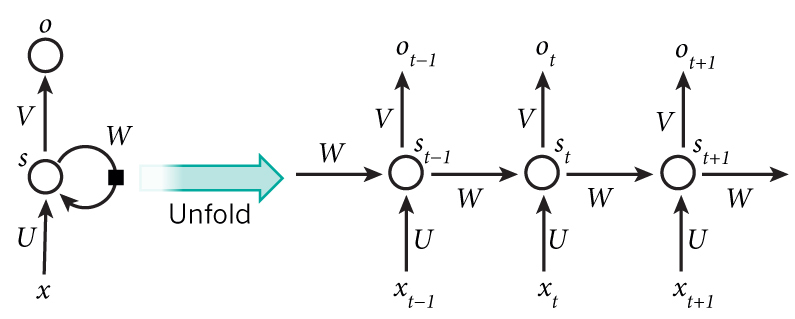
\includegraphics[width=\linewidth]{rnn.jpg}
  \caption{Representation of an RNN, and unfolding the network}
  \label{fig:rnn}
\end{figure}

As can be seen in the figure, the hidden layers have an edge to itself, meaning the hidden layer takes inputs from the input layer and the hidden layer from the previous timestep. It is equivalent to the unrolled neural network as shown in the figure.

In the figure, xt is the input at time step t. st is the hidden state at step t. st is calculated as follows:

st = f(Uxt + Wst-1)

where U, V, W are the corresponding weights as shown in the figure.

The function f is an activation function like tanh. ot is the output at step t.

The neural network uses the backpropagation through time algorithm for learning the weights U,V and W.

\subsection{Long Short Term Memory Networks}

RNNs generally have difficulties in learning long-range sequential data. This is often attributed to the \emph{Vanishing Gradient problem}, which arises because of the chosen activation function(tanh). The deriviatives of tanh function are in the range (-1,1), and because backpropagation computes gradients using chain rule, it involves multiplying these deriviatives. This has the effect of obtaining a deriviative that is so small that the network is not able to learn long range data.

This problem can be solved by using an activation function like ReLU (rectifier) whose deriviatives are constants of either 0 or 1.

Another solution is to use an LSTM, which are specially designed recurrent neural networks capable of learning long term data.

\subsection{Generative Adversarial Networks}
Generative adversarial networks are a branch of unsupervised machine learning, implemented by a system of two neural networks competing against each other. In context of music generation, one network acts as the “forger” network, a network that aims to generate new pieces of music, one is the “discriminator” network, a network that aims to discriminate between low rated music and high rated music. Both the networks work in tandem, fighting each other for accuracy and improving each other in the process, to the point where the “forger” network is so good that it becomes difficult for the “discriminator” network or even a normal human being to catch whether the musical piece has been conceived naturally or artificially.
\section{Model}
\subsection{ABC notation}
The initial recurrent neural network uses abc notation as input. ABC notation is a shorthand form of musical notation. In basic form it uses the letters A through G to represent the given notes, with other elements used to place added value on these - sharp, flat, the length of the note, key, ornamentation. Since ABC notation is in essence a textual data, a character level recurrent neural network, which takes as input individual characters at a time can be created.

The dataset comprises of 1000 tunes scraped from The Nottingham Music database : http://ifdo.ca/~seymour/nottingham/nottingham.html. The abc notation of each tune was concatenated to get a single training data file.

abc2midi program has been used to convert the generated abc notation to midi files. timidity program has been used to play these midi files.

\subsection{Character Level Model}
A recurrent neural network, whose input and output consists of only a single character is called a character level model. Following this representation, a recurrent neural network may be created for virtually any kind of textual data. Historically, similar models have been tried out for various kind of data sets, such as -
\begin{itemize}
\item Shakespeare's Plays
\item Wikipedia Articles
\item HTML documents
\item LATEX documents
\item C++ code
\item Research Papers
\item Music
\end{itemize}

These models were able to generate documents that \emph{looked} similar to the training documents, however sometimes the network wasn't able to capture subtleties like the grammar/format involved with a particular type of document.

\subsection{Music Generation Model - Recurrent Neural Networks}
The first model that has been tried uses a simple recurrent neural network, with backpropagation through time (BPTT) algorithm as the learning algorithm. The code has been implemented in python, using the chainer library for using parallel implementations of the algorithm.

The network uses a single hidden layer with 128 neurons. The input layer and output layer both consist of 93 neurons each, corresponding to 93 different types of characters used in abc notation. The input layer contains one neuron for each different symbol, with a value of one if that particular character is used, otherwise 0. 

The network has been trained for 50 epochs, and the inital learning rate is 2e-3. The learning rate decays after every 10 epochs, with a decay rate of 0.95.

The network, after the training phase can accept a seed string and use it to predict the next few characters.

\section{Results and Analysis}


\begin{figure}
  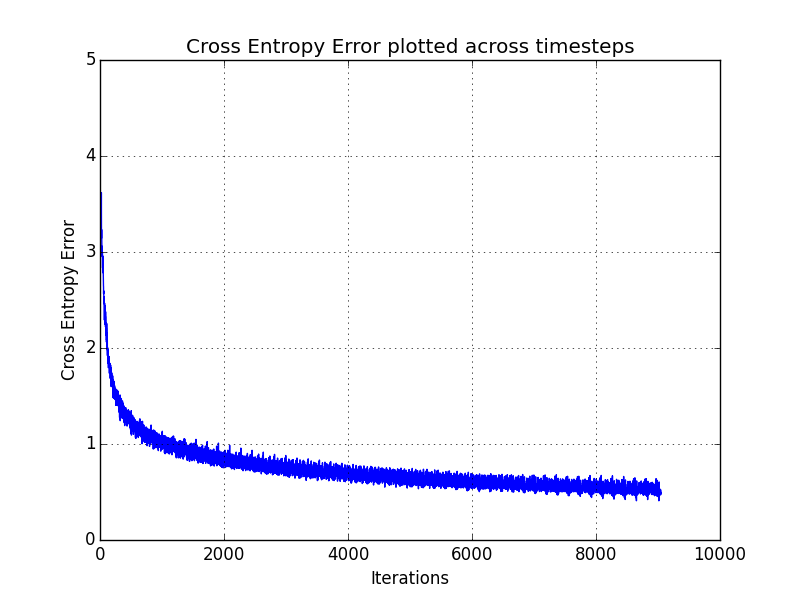
\includegraphics[width=\linewidth]{graph.png}
  \caption{Plot of the cross entropy error across iterations}
  \label{fig:graph}
\end{figure}

The model uses cross entropy error as the function to minimise using backpropagation through time algorithm. The initial cross entropy error is 4.5, and after training the network on 1000 tunes, this cross entropy error comes down to 0.45.

It was found that \emph{long} seed strings that comply with the grammar and notation style of the abc notation give better results.

The recurrent neural network is able to generate musical pieces, however, it can be observed that the rhythm produced is repetitive, implying that the network is not able to learn over long sequences, and their is not much of a variety in the musical pieces generated.

Also, while the network is able to generate abc notation that looks similar to a human in comparison to other notations, the network is not able to capture the grammar correctly, and the program that has to convert this notation to playable(midi) files highlight these grammatical mistakes.

A sample of generated music in abc notation is shown below - 

\begin{verbatim}

X: 185
T:Sanks's Hornpipe
% Nottingham Music Database
S:via PR
M:4/4
L:1/4
K:B
F/2G/2|"Am"A/2B/2c/2e/2 f/2e/2d/2e/2|fd g/2B/2c/2e/2|a/2^g/2f/2e/2 
d/2e/2g/2e/2|d/2B/2 gc|\
"Am"c/2ag/2 fe|
"Dm"f/2e/2f/2g/2 f/2e/2d/2e/2|"G"f/2e/2d "Am"eg|"D"d/2e/2f/2g/2 "A7"ed/2c/2|\
"G"B3:|

\end{verbatim}
\section{Conclusion}
The primitive recurrent neural network model is able to generate music to a limited satisfaction. It is not able to capture the grammar of the notation correctly, and its generated pieces are repetitive and rather monotonous.

This, however gives a benchmark to test more advanced models against, involving LSTMs or GANs.

\section{Bibliography}
\begin{enumerate}
\item GRUV: Algorithmic Music Generation using
Recurrent Neural Networks: 
\begin{verbatim} https://cs224d.stanford.edu/reports/NayebiAran.pdf
\end{verbatim}
\item Learning the Long-Term Structure of the Blues, Douglas et al 
\begin{verbatim} ftp://ftp.idsia.ch/pub/juergen/2002_icannMusic.pdf

\end{verbatim}
\item Daniel Johnson's Blog for music generation using RNN :
\begin{verbatim} http://www.hexahedria.com/2015/08/03/composing-music
-with-recurrent-neural-networks/

\end{verbatim}
\item Andrej Kerpathy - Unreasonable effectiveness of Recurrent Neural Networks 
\begin{verbatim}http://karpathy.github.io/2015/05/21/rnn-effectiveness/

\end{verbatim}
\item Generative Adversarial Networks 
\begin{verbatim}https://arxiv.org/pdf/1602.05110v5.pdf

\end{verbatim}
\end{enumerate}
\end{document}